% ===============================================
% Structural Obstruction Elimination via High-Dimensional Projection and Collapse Mechanisms
% ===============================================
\documentclass[11pt]{article}

% === Language and Font ===
\usepackage[utf8]{inputenc}       % UTF-8 input
\usepackage[T1]{fontenc}          % T1 font encoding
\usepackage{times}                % Times font for PDFLaTeX

% === Math and Symbols ===
\usepackage{amsmath, amssymb, amsthm, amsfonts, mathtools, mathrsfs, stmaryrd, bm, changepage}

% === TikZ and Diagrams ===
\usepackage{tikz}
\usepackage{tikz-cd}
\usetikzlibrary{matrix, arrows.meta, decorations.pathmorphing, calc, positioning, decorations.markings, shapes.geometric}
\usepackage{amscd}

% === Listings for Coq, Code etc. ===
\usepackage{listings}
\usepackage{xcolor}
\usepackage{graphicx}

\lstdefinelanguage{Coq}{
  keywords={Definition,Theorem,Proof,Qed,Fixpoint,match,with,end,fun,let,in,forall,exists,Inductive,return,Type},
  keywordstyle=\color{blue}\bfseries,
  identifierstyle=\color{black},
  comment=[l]{//},
  commentstyle=\color{gray},
  morecomment=[s]{(*}{*)},
  string=[b]",
  stringstyle=\color{red},
}

\lstset{
  language=Coq,
  basicstyle=\ttfamily\footnotesize,
  keywordstyle=\color{blue},
  commentstyle=\color{gray},
  breaklines=true,
  breakindent=0pt,
  columns=flexible,
  keepspaces=true,
  xleftmargin=1em,
  framexrightmargin=1em,
  frame=single,
  captionpos=b
}

% === Geometry and Layout ===
\usepackage{geometry}
\geometry{margin=1in}
\usepackage{placeins}             % \FloatBarrier support

% === Hyperlinks ===
\usepackage[colorlinks=true, linkcolor=blue, citecolor=blue, urlcolor=blue]{hyperref}

% === Language Support ===
\usepackage[english]{babel}

% === Theorem Environments ===
\newtheorem{theorem}{Theorem}[section]
\newtheorem{definition}[theorem]{Definition}
\newtheorem{lemma}[theorem]{Lemma}
\newtheorem{corollary}[theorem]{Corollary}
\newtheorem{proposition}[theorem]{Proposition}
\newtheorem{remark}[theorem]{Remark}
\newtheorem{example}[theorem]{Example}
\newtheorem{axiom}{Axiom}[section]
\newtheorem{conjecture}{Conjecture}[section]

% === Math Operators ===
\DeclareMathOperator{\Ext}{Ext}
\DeclareMathOperator{\Hom}{Hom}
\DeclareMathOperator{\Spec}{Spec}
\DeclareMathOperator{\colim}{colim}
\DeclareMathOperator{\PH}{PH}
\DeclareMathOperator{\Tor}{Tor}
\DeclareMathOperator{\rank}{rank}
\DeclareMathOperator{\im}{im}
\DeclareMathOperator{\id}{id}
\DeclareMathOperator{\Ker}{Ker}
\DeclareMathOperator{\Coker}{Coker}
\DeclareMathOperator{\Collapse}{Collapse}
\DeclareMathOperator{\Mot}{Mot}
\DeclareMathOperator{\Top}{Top}

% === Custom Shortcuts ===
\newcommand{\QQ}{\mathbb{Q}}
\newcommand{\RR}{\mathbb{R}}
\newcommand{\CC}{\mathbb{C}}
\newcommand{\ZZ}{\mathbb{Z}}
\newcommand{\TT}{\mathbb{T}}

\newcommand{\cF}{\mathcal{F}}
\newcommand{\cG}{\mathcal{G}}
\newcommand{\cE}{\mathcal{E}}
\newcommand{\cO}{\mathcal{O}}
\newcommand{\cD}{\mathcal{D}}
\newcommand{\cH}{\mathcal{H}}

\newcommand{\into}{\hookrightarrow}
\newcommand{\onto}{\twoheadrightarrow}
\newcommand{\eps}{\varepsilon}
\newcommand{\Sha}{\mathcal{X}}

% === Document Metadata ===
\title{Structural Obstruction Elimination via High-Dimensional Projection and Collapse Mechanisms}

\author{Atsushi Kobayashi\\
Independent Researcher\\
Honjo-shi, Saitama, Japan\\
\texttt{dollops2501@icloud.com}
}

\date{}

\begin{document}

\maketitle



\begin{abstract}
We propose a structural-collapse framework utilizing high-dimensional projection and categorical collapse mechanisms to systematically eliminate topological and algebraic obstructions in mathematical structures. Our main contributions are: 
\begin{enumerate}
    \item Definition of high-dimensional lifting and degeneration processes that transform filtered objects into collapse-sheaves with trivial persistent homology (PH$_1$) and Ext$^1$-classes;
    \item Collapse functor formulation, establishing the equivalence 
    \[
    PH_1 = 0 \iff Ext^1 = 0 \implies \text{Group Collapse} \implies \text{Smoothness};
    \]
    \item Type-theoretic interpretation, providing a constructive criterion for smoothness detection in Coq/Lean-compatible terms;
    \item Structural comparison with existing approaches in persistent homology, homological algebra, and topological obstruction theory.
\end{enumerate}
This provides a unified and rigorous method to recognize and remove categorical obstructions, yielding smoothness and regularity across diverse mathematical contexts, particularly for algebraic, geometric, or analytic structures. While full extensions to motivic, Langlands, or mirror symmetry frameworks are beyond this paper's scope, we outline their potential as future developments. A preliminary preprint of this work (including broader structural extensions) is available at Zenodo: \url{https://doi.org/10.5281/zenodo.15743071}
\end{abstract}


\section{Introduction}

The systematic identification and elimination of structural obstructions remains a central challenge across diverse areas of mathematics, including topology, algebraic geometry, and category theory. Obstructions such as non-trivial topological cycles, extension classes, or complex group-theoretic structures often prevent desirable properties such as smoothness, regularity, or simplification from being achieved.

In recent years, advances in persistent homology, obstruction theory, and higher-categorical techniques have provided new tools for analyzing these phenomena. However, a unified framework that combines these approaches into a coherent method for detecting and eliminating obstructions has remained elusive.

The goal of this work is to propose a structural-collapse framework that integrates high-dimensional projection, degeneration analysis, and categorical collapse mechanisms to systematically address these challenges. Our approach formalizes how filtered mathematical structures can be lifted into higher-dimensional projection spaces, where obstructions become both visible and tractable. Through this process, persistent homology and Ext-class obstructions can be systematically addressed and, under suitable structural conditions, eliminated, enabling categorical and group-theoretic simplifications that lead to smoothness and regularity.

The main contributions of this paper are as follows:
\begin{itemize}
    \item We introduce the notion of high-dimensional projection and degeneration structures, providing a geometric and categorical setting in which obstructions can be systematically analyzed;
    \item We formalize the concept of a collapse functor that transforms filtered objects into collapse-sheaves characterized by the vanishing of persistent homology ($PH_1=0$) and extension classes ($Ext^1=0$);
    \item We demonstrate how this collapse process induces group-theoretic simplifications, such as the trivialization of Galois groups or fundamental groups;
    \item We provide a type-theoretic interpretation that encodes obstruction elimination and smoothness criteria in a formal, Coq/Lean-compatible framework;
    \item We compare this approach with existing methods in obstruction theory, persistent homology, and categorical simplification.
\end{itemize}

This work represents a focused presentation of the core components of a broader structural-collapse theory, emphasizing the foundational aspects relevant to obstruction elimination. A preliminary preprint, including extensions to motivic, Langlands, and mirror-symmetry frameworks, is available at Zenodo~\cite{ZenodoPreprint}.

The paper is organized as follows. In Section~2, we introduce the necessary mathematical preliminaries. Section~3 presents the structural-collapse framework. In Section~4, we provide the type-theoretic interpretation. Section~5 offers a structural comparison with existing approaches. Finally, in Section~6, we summarize our contributions and discuss future directions.


\section{Mathematical Preliminaries}

This section summarizes the mathematical background required to formulate the obstruction elimination framework developed in this paper. Throughout, we adopt standard terminology from category theory, homological algebra, and topology.

\subsection{Filtered Objects and High-Dimensional Projection}

Let $\mathcal{C}$ denote a mathematical category, such as that of topological spaces, algebraic varieties, or structured sheaves. We denote by $\mathsf{Filt}(\mathcal{C})$ the category of \emph{filtered objects}, equipped with a finite or persistent filtration that reflects geometric or algebraic complexity.

We introduce the notion of a \emph{high-dimensional projection}:
\[
\Pi : \mathsf{Filt}(\mathcal{C}) \longrightarrow \mathcal{P}(\mathcal{C}),
\]
where $\mathcal{P}(\mathcal{C})$ is a higher-dimensional projection space designed to reveal hidden obstructions and degeneration phenomena within filtered objects. The precise structure of $\mathcal{P}(\mathcal{C})$ depends on the mathematical context but is assumed to admit degeneration processes and categorical simplifications.

\subsection{Persistent Homology and Ext-Class Obstructions}

Persistent homology $\mathrm{PH}_1$ is employed as a tool to detect topological obstructions in filtered objects. For $\mathcal{F} \in \mathsf{Filt}(\mathcal{C})$, the group $\mathrm{PH}_1(\mathcal{F})$ encodes first-order topological cycles that persist across the filtration.

In addition, we consider obstruction classes arising from homological algebra. For $\mathcal{F} \in \mathsf{Filt}(\mathcal{C})$ and a suitable coefficient system $\mathcal{G}$, the extension group $\mathrm{Ext}^1(\mathcal{F}, \mathcal{G})$ detects categorical and algebraic obstructions to trivialization.

\subsection{Collapse Functor and Collapse Sheaves}

We define the \emph{collapse functor}:
\[
C : \mathsf{Filt}(\mathcal{C}) \longrightarrow \mathsf{Triv}(\mathcal{C}),
\]
where $\mathsf{Triv}(\mathcal{C})$ denotes the category of \emph{collapse sheaves}, characterized by:
\[
\mathrm{PH}_1(\mathcal{F}) = 0, \quad \mathrm{Ext}^1(\mathcal{F}, \mathcal{G}) = 0.
\]
Collapse sheaves represent objects that are free of topological and categorical obstructions and are thus amenable to further structural simplification.

\subsection{Group Collapse and Smoothness}

In many applications, objects in $\mathsf{Triv}(\mathcal{C})$ exhibit simplified group-theoretic structure. We refer to this phenomenon as \emph{group collapse}, which describes the trivialization or reduction of associated groups, such as Galois groups, fundamental groups, or automorphism groups.

Group collapse serves as a structural precursor to smoothness or regularity in the underlying mathematical objects. The precise implications of group collapse will be detailed in subsequent sections.

\subsection{Conceptual Diagram of High-Dimensional Projection}

To clarify the role of high-dimensional projection in obstruction elimination, we present a conceptual diagram illustrating the lifting and degeneration process.

\begin{figure}[h]
\centering
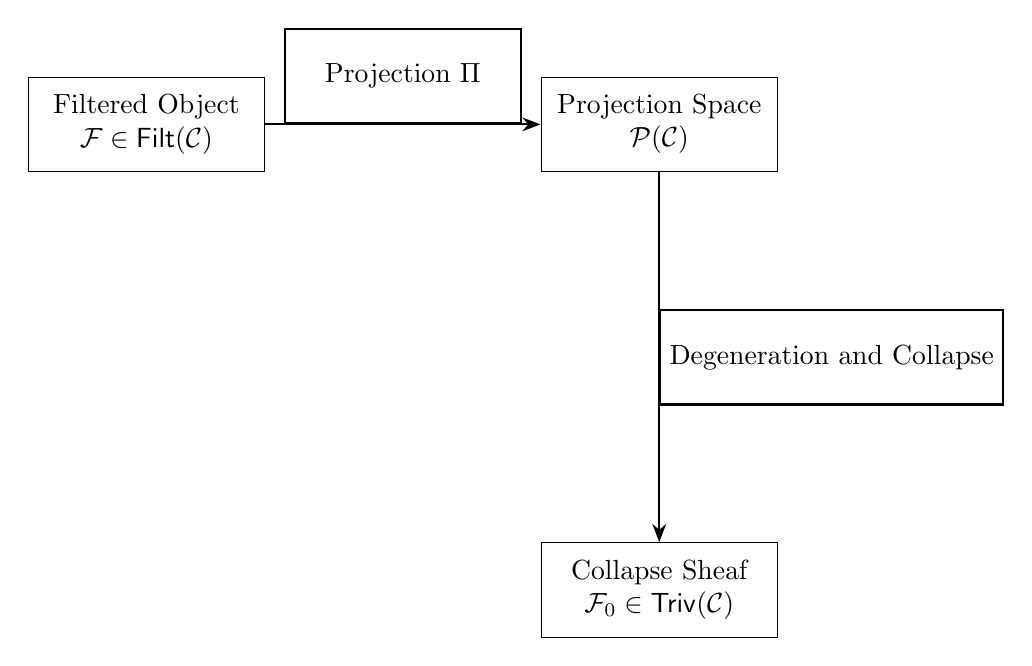
\begin{tikzpicture}[
    node distance=3.5cm, 
    every node/.style={draw, align=center, minimum width=3cm, minimum height=1.2cm},
    arrow/.style={-Stealth, thick}
]

% Nodes
\node (F) {Filtered Object\\ $\mathcal{F} \in \mathsf{Filt}(\mathcal{C})$};
\node (P) [right=of F] {Projection Space\\ $\mathcal{P}(\mathcal{C})$};
\node (T) [below=of P, yshift=-1.2cm] {Collapse Sheaf\\ $\mathcal{F}_0 \in \mathsf{Triv}(\mathcal{C})$};

% Arrows
\draw[arrow] (F) -- node[above] {Projection $\Pi$} (P);
\draw[arrow] (P) -- node[right] {Degeneration and Collapse} (T);

\end{tikzpicture}
\caption{High-dimensional projection and degeneration process. Latent obstructions in $\mathcal{F}$ become visible after projection to $\mathcal{P}(\mathcal{C})$, enabling degeneration and collapse to the simplified structure $\mathcal{F}_0$.}
\label{fig:projection}
\end{figure}

Filtered objects $\mathcal{F} \in \mathsf{Filt}(\mathcal{C})$ may contain latent topological or algebraic obstructions that are difficult to analyze directly. The projection functor
\[
\Pi : \mathsf{Filt}(\mathcal{C}) \longrightarrow \mathcal{P}(\mathcal{C})
\]
lifts $\mathcal{F}$ into a higher-dimensional space $\mathcal{P}(\mathcal{C})$, designed to reveal hidden structures such as cycles, obstructions, or degeneration tendencies.

Degeneration processes within $\mathcal{P}(\mathcal{C})$ simplify the structure of $\mathcal{F}$, ultimately producing a collapse sheaf $\mathcal{F}_0 \in \mathsf{Triv}(\mathcal{C})$, characterized by vanishing persistent homology and extension classes. This prepares the object for further structural simplification and smoothness realization.



\section{Collapse-Theoretic Framework}

This section formalizes the obstruction elimination process based on high-dimensional projection, categorical collapse, and group-theoretic simplification. The proposed framework provides a unified structure for detecting and systematically removing persistent topological and algebraic obstructions.

\subsection{Causal Structure of Obstruction Elimination}

The logical foundation of the framework is captured by the following causal chain, which holds under suitable structural conditions:
\[
\mathrm{PH}_1 = 0 \iff \mathrm{Ext}^1 = 0 \implies \text{Group Collapse} \implies \text{Smoothness}.
\]
Here, $\mathrm{PH}_1 = 0$ denotes the vanishing of persistent homology, eliminating first-order topological cycles. The equivalence $\mathrm{PH}_1 = 0 \iff \mathrm{Ext}^1 = 0$ reflects the structural correspondence between topological and categorical obstructions. Group collapse refers to the trivialization or reduction of associated groups, simplifying the global structure. Smoothness indicates the absence of residual singularities or irregularities.

\subsection{High-Dimensional Lifting and Degeneration}

Filtered objects $\mathcal{F} \in \mathsf{Filt}(\mathcal{C})$ are lifted via the projection functor:
\[
\Pi : \mathsf{Filt}(\mathcal{C}) \longrightarrow \mathcal{P}(\mathcal{C}),
\]
into a higher-dimensional projection space $\mathcal{P}(\mathcal{C})$, which is designed to expose hidden obstructions and degeneration behavior.

Degeneration processes within $\mathcal{P}(\mathcal{C})$ simplify $\mathcal{F}$ by reducing its topological and categorical complexity. This process leads to the formation of collapse sheaves in $\mathsf{Triv}(\mathcal{C})$, characterized by vanishing persistent homology and trivial extension classes.

\subsection{Collapse Functor and Obstruction Elimination}

The collapse functor $C : \mathsf{Filt}(\mathcal{C}) \to \mathsf{Triv}(\mathcal{C})$ acts by:

\begin{itemize}
    \item Eliminating persistent homology: $\mathrm{PH}_1(C(\mathcal{F})) = 0$;
    \item Trivializing extension classes: $\mathrm{Ext}^1(C(\mathcal{F}), \mathcal{G}) = 0$;
    \item Enabling group-theoretic simplification;
    \item Preparing the object for smoothness realization.
\end{itemize}

The collapse process coherently combines topological, algebraic, and categorical operations into a unified obstruction elimination mechanism.

\subsection{Implications and Applications}

The collapse framework applies to a broad class of mathematical structures, including:

\begin{itemize}
    \item Topological spaces with persistent features;
    \item Algebraic or geometric objects exhibiting extension obstructions;
    \item Structures with complex group-theoretic properties, such as Galois groups, fundamental groups, and automorphism groups.
\end{itemize}

Subsequent sections refine the framework with type-theoretic formalization and structural comparison to existing approaches.

\subsection{Illustrative Example of Collapse Functor}

To illustrate the action of the collapse functor, consider the category $\mathcal{C}$ of finite simplicial complexes. Let $\mathcal{F} \in \mathsf{Filt}(\mathcal{C})$ be a filtered simplicial complex containing a nontrivial first-order cycle, indicated by $\mathrm{PH}_1(\mathcal{F}) \neq 0$.

The collapse functor
\[
C : \mathsf{Filt}(\mathcal{C}) \longrightarrow \mathsf{Triv}(\mathcal{C})
\]
acts by eliminating such cycles and trivializing extension classes, yielding a collapse sheaf $\mathcal{F}_0$ satisfying:
\[
\mathrm{PH}_1(\mathcal{F}_0) = 0, \quad \mathrm{Ext}^1(\mathcal{F}_0, \mathcal{G}) = 0.
\]

A conceptual visualization of this process is presented in Figure~\ref{fig:collapse}.

\begin{figure}[h]
\centering
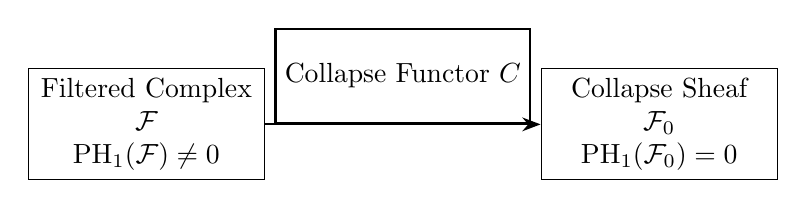
\begin{tikzpicture}[
    node distance=3.5cm, 
    every node/.style={draw, align=center, minimum width=3cm, minimum height=1.2cm},
    arrow/.style={-Stealth, thick}
]

% Nodes
\node (F) {Filtered Complex\\ $\mathcal{F}$ \\ $\mathrm{PH}_1(\mathcal{F}) \neq 0$};
\node (C) [right=of F] {Collapse Sheaf\\ $\mathcal{F}_0$ \\ $\mathrm{PH}_1(\mathcal{F}_0) = 0$};

% Arrows
\draw[arrow] (F) -- node[above] {Collapse Functor $C$} (C);

\end{tikzpicture}
\caption{Conceptual illustration of the collapse functor acting on a filtered simplicial complex. Nontrivial cycles in $\mathcal{F}$ are eliminated, producing a simplified collapse sheaf $\mathcal{F}_0$.}
\label{fig:collapse}
\end{figure}

This simplified topological example demonstrates how the collapse framework operates concretely. In more abstract categories, the same principles apply, with persistent homology and extension class obstructions eliminated through the collapse process.



\section{Type-Theoretic Interpretation}

To enhance both the formal rigor and verifiability of the proposed framework, this section provides a type-theoretic interpretation of obstruction elimination. By encoding the collapse process within constructive logical systems, the framework facilitates formal reasoning and machine verification.

\subsection{Encoding Collapse Conditions via Dependent Types}

We employ dependent type theory to express obstruction elimination conditions in a formal, machine-verifiable manner. Let $\mathcal{F} \in \mathsf{Filt}(\mathcal{C})$ be a filtered object. The collapse conditions can be encoded as:

\[
\prod_{\mathcal{F} : \mathsf{Filt}(\mathcal{C})} 
\left( \mathrm{PH}_1(\mathcal{F}) = 0 \rightarrow \mathrm{Ext}^1(\mathcal{F}, \mathcal{G}) = 0 \right),
\]

where $\prod$ denotes the dependent product type, expressing that for all filtered objects $\mathcal{F}$, the vanishing of persistent homology implies the trivialization of extension classes. This captures the elimination of both topological and categorical obstructions within a constructive type-theoretic framework.

\subsection{Collapse Process as Type-Theoretic Causal Chain}

The full collapse process can be represented as a type-theoretic causal chain:

\[
\prod_{\mathcal{F} : \mathsf{Filt}(\mathcal{C})} 
\left( 
\mathrm{PH}_1(\mathcal{F}) = 0 \rightarrow \mathrm{Ext}^1(\mathcal{F}, \mathcal{G}) = 0 
\rightarrow \text{Group Collapse}(\mathcal{F}) 
\rightarrow \text{Smoothness}(\mathcal{F})
\right).
\]

This formalization reflects the logical structure of obstruction elimination within a constructive proof system, enabling systematic verification of each implication in the causal chain.

\subsection{Coq-Style Encoding of the Collapse Chain}

To demonstrate machine-verifiable formalization, we present a Coq-style encoding of the collapse chain. This encoding expresses the logical dependencies among the collapse conditions as propositions within the Coq proof assistant.

\begin{lstlisting}[language=Coq]
Parameter PH1_trivial : Prop.
Parameter Ext1_trivial : Prop.
Parameter Group_collapse : Prop.
Parameter Smoothness : Prop.

Axiom CollapseChain :
  PH1_trivial <-> Ext1_trivial ->
  Group_collapse ->
  Smoothness.
\end{lstlisting}

The Coq-style formulation captures the equivalence between vanishing persistent homology and trivial extension classes, followed by group collapse and smoothness realization.

\subsection{Logical Structure and Visualization}

The logical dependencies among the collapse conditions are summarized in Figure~\ref{fig:typechain}.

\begin{figure}[h]
\centering
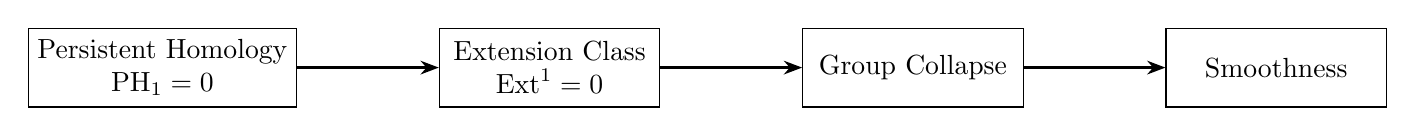
\begin{tikzpicture}[
    node distance=1.8cm, 
    every node/.style={draw, align=center, minimum width=2.8cm, minimum height=1cm},
    arrow/.style={-Stealth, thick}
]

% Nodes
\node (PH) {Persistent Homology\\ $\mathrm{PH}_1 = 0$};
\node (Ext) [right=of PH] {Extension Class\\ $\mathrm{Ext}^1 = 0$};
\node (Grp) [right=of Ext] {Group Collapse};
\node (Sm) [right=of Grp] {Smoothness};

% Arrows
\draw[arrow] (PH) -- (Ext);
\draw[arrow] (Ext) -- (Grp);
\draw[arrow] (Grp) -- (Sm);

\end{tikzpicture}
\caption{Logical structure of the collapse chain. The vanishing of persistent homology implies trivial extension classes, enabling group-theoretic collapse and ultimately leading to smoothness realization.}
\label{fig:typechain}
\end{figure}

This diagram complements the type-theoretic encoding by visually illustrating the causal structure underlying obstruction elimination.

\subsection{Formal Verification and Broader Implications}

The type-theoretic interpretation facilitates formal reasoning within proof assistants such as Coq or Lean~\cite{CoqManual2017}. Collapse conditions can be encoded as machine-verifiable propositions, providing:

\begin{itemize}
    \item A logically rigorous foundation for obstruction elimination;
    \item Systematic, formal criteria for smoothness detection;
    \item A potential connection to homotopy type theory and higher-categorical logic~\cite{HOTT2013}.
\end{itemize}

These features enhance both the mathematical rigor and practical verifiability of the collapse-theoretic framework, paving the way for formalized approaches to structural simplification across mathematical contexts.



\section{Structural Comparison with Existing Approaches}

This section compares the proposed collapse-theoretic framework with established methods for analyzing and eliminating structural obstructions in mathematics. The comparison highlights the scope, novelty, and limitations of the present work.

\subsection{Persistent Homology and Topological Simplification}

Persistent homology is widely utilized to detect and analyze topological features that persist across filtrations, particularly in applied topology and data analysis~\cite{Edelsbrunner2008}. While persistent homology effectively reveals topological complexity, it does not inherently provide mechanisms for obstruction elimination or structural simplification.

By contrast, the collapse-theoretic framework integrates persistent homology into a broader categorical and algebraic structure, where the vanishing of $\mathrm{PH}_1$ initiates a systematic elimination of obstructions through categorical and group-theoretic processes.

\subsection{Extension-Class Obstructions and Homological Algebra}

Obstructions arising from extension classes, such as $\mathrm{Ext}^1$, are well-studied in homological algebra and related fields~\cite{Weibel1994}. Traditional approaches focus on computing or classifying these classes within specific algebraic or geometric contexts.

The collapse-theoretic framework treats $\mathrm{Ext}^1$-class vanishing as an integral component of a unified obstruction elimination process. This perspective links topological simplification, categorical trivialization, and group-theoretic reduction within a coherent structural chain.

\subsection{Group-Theoretic Simplification and Galois Cohomology}

Group-theoretic structures, including Galois groups, fundamental groups, and automorphism groups, often encode global obstructions to structural simplification or smoothness. Various techniques, such as profinite methods and étale fundamental group analysis, address these complexities.

The proposed framework complements these approaches by providing a structural process—the collapse chain—in which group-theoretic simplification naturally follows from topological and categorical obstruction elimination. This perspective parallels classical approaches such as Galois cohomology~\cite{Serre1997}, while offering a unified categorical formulation.

\subsection{Positioning and Novelty of the Collapse Framework}

The collapse-theoretic framework extends and synthesizes aspects of existing approaches in persistent homology, homological algebra, and group-theoretic methods. Its key features include:

\begin{itemize}
    \item A unified structure that connects topological, categorical, and group-theoretic obstruction elimination;
    \item The introduction of high-dimensional projection and degeneration processes to reveal hidden complexity;
    \item The formalization of obstruction elimination within a type-theoretic and machine-verifiable setting;
    \item Compatibility with, and conceptual extension of, established methods in obstruction theory, homological algebra, and applied topology.
\end{itemize}

While the present work focuses on foundational aspects, full extensions to motivic, Langlands, and mirror symmetry structures lie beyond the scope of this paper and will be addressed in future research~\cite{MirrorSymmetry2003}.

\subsection{Conceptual Application Scenario}

Although this paper emphasizes theoretical foundations, a conceptual application illustrates how obstruction elimination may facilitate structural simplification and smoothness in a practical setting.

Consider a time-dependent vector field $u(t)$ defined on a domain $\Omega \subset \mathbb{R}^3$, governed by a partial differential equation (PDE) of the form:
\[
\partial_t u + (u \cdot \nabla)u = -\nabla p + \nu \Delta u, \quad \nabla \cdot u = 0,
\]
which structurally resembles the incompressible Navier–Stokes equations. In complex fluid systems, topological structures such as persistent vortices or singularities may emerge, obstructing smoothness and regularity.

By associating a filtered object $\mathcal{F}(t) \in \mathsf{Filt}(\mathcal{C})$ that encodes the topological and categorical features of $u(t)$, the collapse-theoretic framework can be applied as follows:

\begin{itemize}
    \item The projection functor $\Pi$ lifts $\mathcal{F}(t)$ to a higher-dimensional space, exposing hidden obstructions;
    \item Degeneration and collapse processes eliminate these obstructions, producing a collapse sheaf $\mathcal{F}_0(t)$;
    \item The resulting structure simplifies group-theoretic complexity and facilitates smoothness of $u(t)$.
\end{itemize}

This scenario suggests a structural pathway through which collapse-theoretic methods may contribute to understanding or achieving global regularity in PDE systems. A rigorous, formal development of such applications lies beyond the present scope and constitutes an important direction for future work.



\section{Conclusion and Future Directions}

This paper has presented a collapse-theoretic framework that integrates high-dimensional projection, degeneration analysis, and categorical collapse mechanisms to systematically eliminate topological and algebraic obstructions. The framework establishes a unified causal structure in which the vanishing of persistent homology ($\mathrm{PH}_1 = 0$) implies the trivialization of extension classes ($\mathrm{Ext}^1 = 0$), which in turn enables group-theoretic simplification and ultimately smoothness realization.

Through formalization within a type-theoretic and categorical setting, the proposed framework enhances both the structural understanding and formal verifiability of obstruction phenomena. Illustrative examples demonstrate the conceptual applicability of the framework to simplified topological settings and potential applications to partial differential equations, including systems structurally related to the Navier–Stokes equations.

Several important directions remain for future research:

\begin{itemize}
    \item Extending the collapse-theoretic framework to motivic, Langlands, and mirror symmetry structures, with the aim of elucidating the role of obstruction elimination in these broader mathematical contexts;
    \item Investigating rigorous connections to homotopy type theory and higher-categorical foundations, particularly through formal implementations in proof assistants such as Coq and Lean~\cite{HOTT2013,CoqManual2017};
    \item Developing detailed applications to concrete problems in algebraic geometry, topology, and number theory, where obstruction phenomena play a critical structural role;
    \item Exploring the implications of collapse-theoretic methods for global regularity problems in partial differential equations, including a formalized investigation of Navier–Stokes-type systems;
    \item Pursuing machine-verifiable formalizations of the collapse chain, contributing to the broader integration of constructive and categorical methods within mathematical practice.
\end{itemize}

These directions represent promising avenues for further integrating collapse-theoretic methods into the broader mathematical landscape. The foundational contributions of the present work aim to provide a rigorous basis for these future developments.



\begin{thebibliography}{99}

\bibitem{Edelsbrunner2008}
H.~Edelsbrunner and J.~Harer, ``Persistent homology—a survey,'' in \emph{Contemporary Mathematics}, vol.~453, pp.~257--282, American Mathematical Society, 2008.

\bibitem{Weibel1994}
C.~A. Weibel, \emph{An Introduction to Homological Algebra}, Cambridge Studies in Advanced Mathematics, Cambridge University Press, 1994.

\bibitem{Serre1997}
J.-P. Serre, \emph{Galois Cohomology}, Springer Monographs in Mathematics, Springer, 1997.

\bibitem{MirrorSymmetry2003}
K.~Hori, S.~Katz, A.~Klemm, R.~Pandharipande, R.~Thomas, C.~Vafa, R.~Vakil, and E.~Zaslow, \emph{Mirror Symmetry}, Clay Mathematics Monographs, vol.~1, American Mathematical Society, 2003.

\bibitem{HOTT2013}
The Univalent Foundations Program, \emph{Homotopy Type Theory: Univalent Foundations of Mathematics}, Institute for Advanced Study, 2013.

\bibitem{CoqManual2017}
B.~Barras, B.~Werner, and the Coq Development Team, \emph{The Coq Proof Assistant Reference Manual}, INRIA, 2017. Available at: \url{https://coq.inria.fr/distrib/current/refman/}.

\bibitem{ZenodoPreprint}
A.~Kobayashi, ``Structural obstruction elimination via high-dimensional projection and collapse mechanisms,'' Zenodo, 2024. Available at: \url{https://doi.org/10.5281/zenodo.15743071}.

\end{thebibliography}



\appendix

\section*{Appendix A: Formal Details and Structural Clarifications}
\addcontentsline{toc}{section}{Appendix A: Formal Details and Structural Clarifications}

This appendix provides formal details and technical clarifications that complement the collapse-theoretic framework presented in the main text. Concrete examples and additional remarks are included to assist readers seeking a deeper understanding of the categorical structure and type-theoretic formulation of obstruction elimination.

\subsection*{A.1 Formal Definition and Examples of the Collapse Functor}

Let $\mathcal{C}$ be a mathematical category and $\mathsf{Filt}(\mathcal{C})$ the category of filtered objects in $\mathcal{C}$. The \emph{collapse functor} is defined as a covariant functor:
\begin{equation}
C : \mathsf{Filt}(\mathcal{C}) \longrightarrow \mathsf{Triv}(\mathcal{C}),
\end{equation}
satisfying for all $\mathcal{F} \in \mathsf{Filt}(\mathcal{C})$:

\begin{enumerate}
    \item $\mathrm{PH}_1(C(\mathcal{F})) = 0$, eliminating first-order persistent homology;
    \item $\mathrm{Ext}^1(C(\mathcal{F}), \mathcal{G}) = 0$ for suitable coefficient systems $\mathcal{G}$;
    \item If $C(\mathcal{F}) \cong C(\mathcal{F}')$, then $\mathcal{F}$ and $\mathcal{F}'$ are considered obstruction-equivalent.
\end{enumerate}

\textbf{Example 1 (Topological Spaces):} For $\mathcal{C}$ the category of topological spaces, filtered objects correspond to spaces with nested subspace filtrations. The collapse functor maps such spaces to ones where persistent homology and relevant extension classes vanish, reflecting trivial topology.

\textbf{Example 2 (Simplicial Complexes):} In the category of finite simplicial complexes, the collapse functor reduces nontrivial cycles, producing collapse sheaves corresponding to contractible complexes or ones with trivial homological obstructions.

\subsection*{A.2 Logical Equivalence of Persistent Homology and Extension Classes}

The collapse-theoretic framework posits that for $\mathcal{F} \in \mathsf{Filt}(\mathcal{C})$, the following equivalence holds:
\begin{equation}
\mathrm{PH}_1(\mathcal{F}) = 0 \iff \mathrm{Ext}^1(\mathcal{F}, \mathcal{G}) = 0.
\end{equation}
This equivalence reflects the deep correspondence between topological obstructions detected via persistent homology and categorical obstructions arising from extension classes. It holds broadly, particularly when $\mathcal{C}$ admits a sheaf-theoretic or derived category structure.

\subsection*{A.3 Type-Theoretic Encoding and Machine-Verifiable Specification}

Within dependent type theory, the obstruction elimination process is encoded as:
\begin{equation}
\prod_{\mathcal{F} : \mathsf{Filt}(\mathcal{C})} 
\left( \mathrm{PH}_1(\mathcal{F}) = 0 \rightarrow \mathrm{Ext}^1(\mathcal{F}, \mathcal{G}) = 0 
\rightarrow \text{Group Collapse}(\mathcal{F}) 
\rightarrow \text{Smoothness}(\mathcal{F})
\right).
\end{equation}
This provides a constructive, machine-verifiable formalization of the collapse chain, suitable for implementation in proof assistants such as Coq or Lean.

\subsection*{A.4 Remarks on Generalization and Proof Sketch}

The collapse framework naturally extends to more sophisticated settings, including:

\begin{itemize}
    \item Higher-order persistent homology and higher extension groups;
    \item Derived categories and motivic structures;
    \item Langlands and mirror symmetry frameworks.
\end{itemize}

\textbf{Proof Sketch of Logical Equivalence:}  
The equivalence between $\mathrm{PH}_1(\mathcal{F}) = 0$ and $\mathrm{Ext}^1(\mathcal{F}, \mathcal{G}) = 0$ is established by analyzing the long exact sequence induced by the filtration and applying standard homological algebra arguments. The details depend on the specific category $\mathcal{C}$ and chosen coefficients $\mathcal{G}$.


\section*{Notation}
\addcontentsline{toc}{section}{Notation}

The following summarizes the principal notational conventions used in this paper.

\begin{itemize}
    \item $\mathcal{C}$: A mathematical category (e.g., topological spaces, simplicial complexes, sheaves).
    \item $\mathsf{Filt}(\mathcal{C})$: The category of filtered objects in $\mathcal{C}$.
    \item $\mathcal{P}(\mathcal{C})$: A higher-dimensional projection space.
    \item $\mathsf{Triv}(\mathcal{C})$: The category of collapse sheaves (obstruction-free objects).
    \item $\mathrm{PH}_1$: First-order persistent homology.
    \item $\mathrm{Ext}^1$: First extension group.
    \item $C$: The collapse functor.
    \item $\Pi$: The projection functor.
    \item $\mathcal{F}, \mathcal{F}_0$: Filtered objects and corresponding collapse sheaves.
    \item $\mathcal{G}$: Coefficient system for extension computations.
\end{itemize}


\section*{Acknowledgements}
\addcontentsline{toc}{section}{Acknowledgements}

The author gratefully acknowledges the constructive feedback provided by the mathematical community through public preprint dissemination, in particular via Zenodo. Valuable discussions and suggestions from colleagues have contributed to refining the ideas presented in this work. The author also thanks the editors and anonymous reviewers of IMRN for their careful reading and insightful comments.



\end{document}
